To be able to identify the balls, the location of each ball is needed. By knowing where the balls are placed, features from each ball can be extracted and compared for identification.

The location of a ball is defined by the position of the bounding circle of the ball. The radius of a ball is equal  and known for all balls, and the balls can then be represented by the center point alone.

The located positions must be precise to gain the optimal working conditions for the identifier. A ball location that is slightly shifted will result in a ball region that contains pixels which does not come from the ball. This will make it harder for the identifier to identify the ball, and it will become even harder if the region intersects another ball because the region will then become a mix of two different balls. This can cause that the two balls are classified as the other and thereby 2 identification errors.

\subsubsection{Preliminary segmentation}
To decrease the ROI from the cloth area down to areas of the table that contains balls, a preliminary segmentation is performed. A color threshold removes all pixels that belong to the background leaving behind a mask that represents the balls.
\begin{figure}[h]
  \centering
  \subfloat[Original]{\label{fig:gull}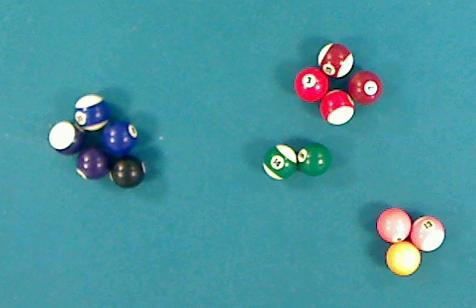
\includegraphics[width=0.48\textwidth]{images/thres1before.jpg}}
  \quad           
  \subfloat[Segmentation]{\label{fig:tiger}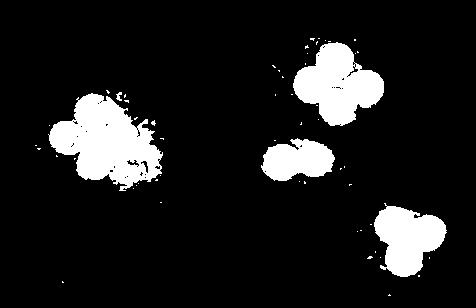
\includegraphics[width=0.48\textwidth]{images/thres1after.jpg}}
   \caption{Color threshold to remove background}
  \label{fig:thres1}
\end{figure}
Figure \ref{fig:thres1} shows the result of the color threshold. In a situation like this where the balls are laying close to each other, the preliminary segmentation is not enough to successfully separate the balls. Balls in close proximity results in connected BLOBs after the threshold. These BLOBs could be separated using morphology operations but most of the information would be lost, causing the locations to lack precision. Instead of using the BLOBS directly, they are used as search regions for the balls.

\subsubsection{Ball detection}
To be able to detect balls in the image, we need to know the features that characterizes a ball. The following description can be formulated:
\begin{itemize}
\item The shape of the ball is always a circle of fixed size
\item The color distribution consists of at least two of three parts:
	\begin{itemize}
		\item White
		\item Black (ball number)
		\item Primary ball color
	\end{itemize}
\end{itemize}
The black and cue balls has black and white, respectively, as their primary color, making them consist of only two distributions, whereas all other balls consists all three. This ball description allows us to formulate a way of measuring the probability of that a given position in the image corresponds to the center of a ball.

If we ignore the black pixels for all balls except for the black(8), the balls only contains 1 primary color and white. The probability of a position containing a ball can then be formulated as
\begin{equation}
P(ball) = \frac{primary + white}{total}
\end{equation}
By finding the non-overlapping positions in the image that maximizes this ratio the balls can be found. Balls are detected at the highest scoring position that does not already contain a ball. The system continues to detect balls until 16 balls are found or the score goes below a threshold. This threshold is set as a ratio of the total pixels in a ball.

\begin{figure}[h]
\begin{center}
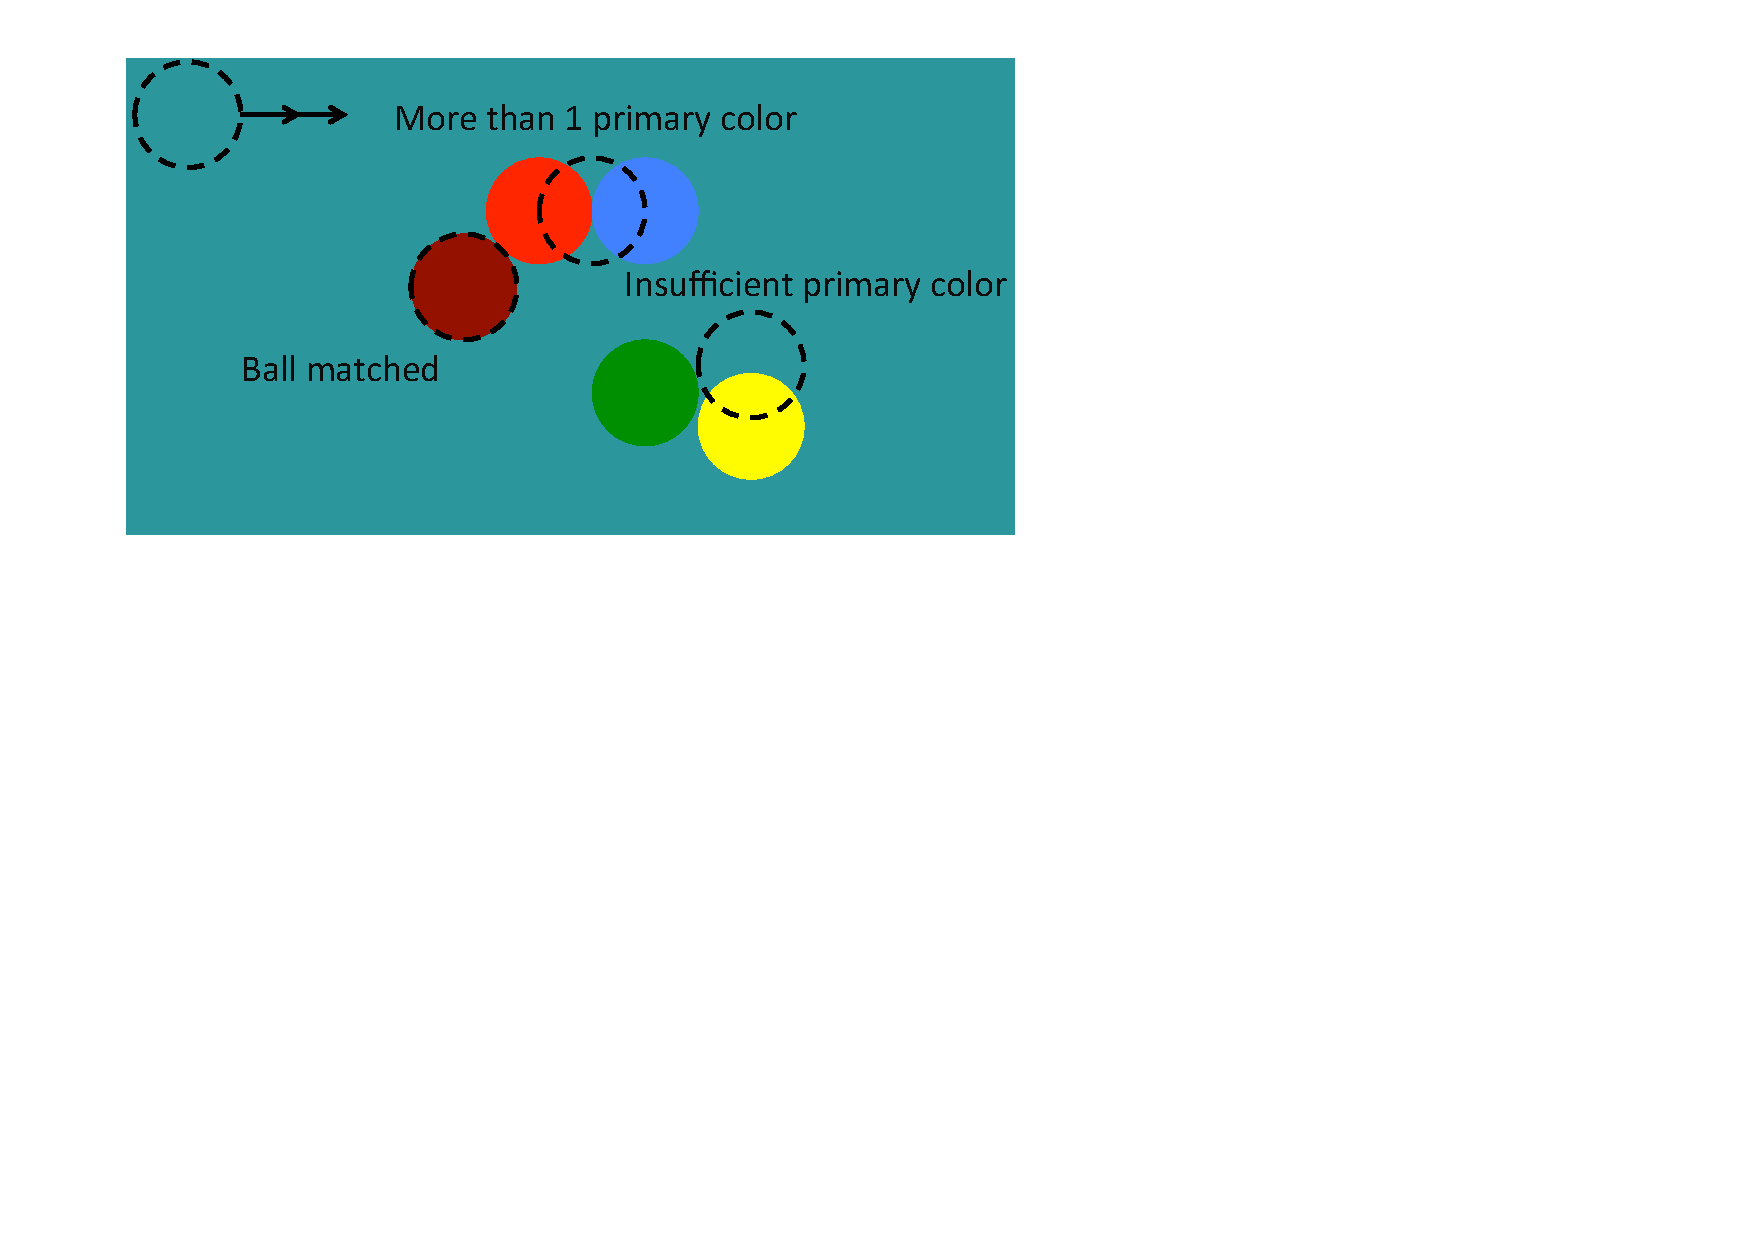
\includegraphics{images/ballfind.pdf}
\caption{The probability of a ball is evaluated in the image.}
\label{fig:ballfind}
\end{center}
\end{figure}
Figure \ref{fig:ballfind} shows the used evaluation method. A circular mask is placed in every position found by the preliminary segmentation. By using a circular patch, the system is able to get a better match against the circular ball regions. Inside the mask an HSV color histogram is computed. All pixels that have a hue value close to the background hue are ignored. The rest of the pixels are sorted into three categories: white pixels, black pixels and primary color. Pixels that have a saturation below a certain value are considered to be white\fixme{Explain?}. Pixels with a value below a threshold are considered to be black. To make the system as color independent as possible, value is only used to identify black pixels. This is necessary because the black color is undefined in hue-saturation space.

If the evaluated position contains a ball, the color distribution in the non-black-or-white pixels is expected to be narrowly distributed around the mean of the ball color. If the position is between two or more balls the distribution will be multimodal and the variance higher. The pixels that are within a certain deviation of the mean hue and saturation are counted, resulting in a count of the number of primary colored pixels in the ball. A ball position will have a high number of pixels that are close to the mean, resulting in a high primary color count. If the number of black pixels are higher than the primary color count, the primary color is set to black.
\fixme{Figure showing different distributions and their resulting ball probability}

As mentioned before, the ball score is computed as the sum of the primary and white pixels. If the score is above the threshold, the ball is saved in a list. When all the positions in the image has been searched, the system iterates through the list to get the final ball positions. The position and the area around  a ballwithin one ball radius is marked as matched. The next ball can then not be found any closer than one radius from the previous matches. A problem arises if a wrong match is found which intersects a not matched ball. It will then be impossible to find a new match in the region of the earlier wrong match.
Figure \ref{fig:wronglocate} shows the problem of a wrong match. The wrong match prevents several balls from being matched, and other balls from matching precisely.
\begin{figure}[h]
\begin{center}
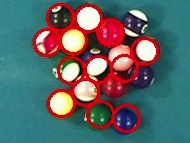
\includegraphics{images/wronglocate.jpg}
\caption{Consequence of wrong location match. Red circles are ball matches}
\label{fig:wronglocate}
\end{center}
\end{figure}